
\documentclass[11pt,a4paper]{article}

\usepackage[utf8]{inputenc} 
\usepackage[T1]{fontenc} 
\usepackage{lmodern}
\usepackage{tcolorbox}

\usepackage[german]{babel}


\setlength{\parindent}{0pt}
\setlength{\parskip}{1ex plus 0.5ex minus 0.5ex}

\usepackage{amsmath} 


\usepackage{graphicx} 

\usepackage[section]{placeins}
\usepackage{booktabs}


\usepackage{hyperref}
\hypersetup{
	colorlinks,
	citecolor=red,
	filecolor=black,
	linkcolor=black,
	urlcolor=black}
\graphicspath{}

\begin{document}
	

{
	\centering 
	\large 
	Physiklabor für Anfänger*innen \\
	Ferienpraktikum im Sommersemester 2018 \\[4mm]
	\textbf{\LARGE 
		Versuch 8: Viskosität aus dem Durchströmen einer Kapillare
	} \\[3mm]
	(durchgeführt am 26.09.2018 bei Pascal) \\
	Ye Joon Kim, Marouan Zouari\\
	\today \\[10mm]
}
\tableofcontents

\section{Aufbau}


\section{Durchführung}

\section{Auswertung und Fehleranalyse}
Zur Bestimmung der Viskosität wurde die folgende Formel benutzt:
\begin{equation}
	I_V = \frac{V}{t} = \frac{\pi R^4 \Delta p}{8 \eta l}
\end{equation}
Die Druckdifferenz lässt sich mit:
$$\Delta p = \rho_w hg$$
bestimmen. Deswegen bei einer Auftragung von $I_V$ gegen $\frac{R^4}{l}$ entspricht die Steigung dem Wert $\frac{ \pi \rho_w hg}{8\eta}$.

Da der Zusammenhang lässt sich in einer Form von $I_V = a + b(\frac{R^4}{l})$ schreiben lässt, wurden die Werte für $I_V$ dann in einer Graph mit dem Programm Logger Pro gegen $\frac{R^4}{l}$ aufgetragen (Siehe Abbildung(2)). Die Werte für $a$, der Achsenabschnitt, $b$, die Steigung, und deren Unsicherheiten wurden mit einem Excel-Dokument berechnet. 

\begin{figure}
	\centering
	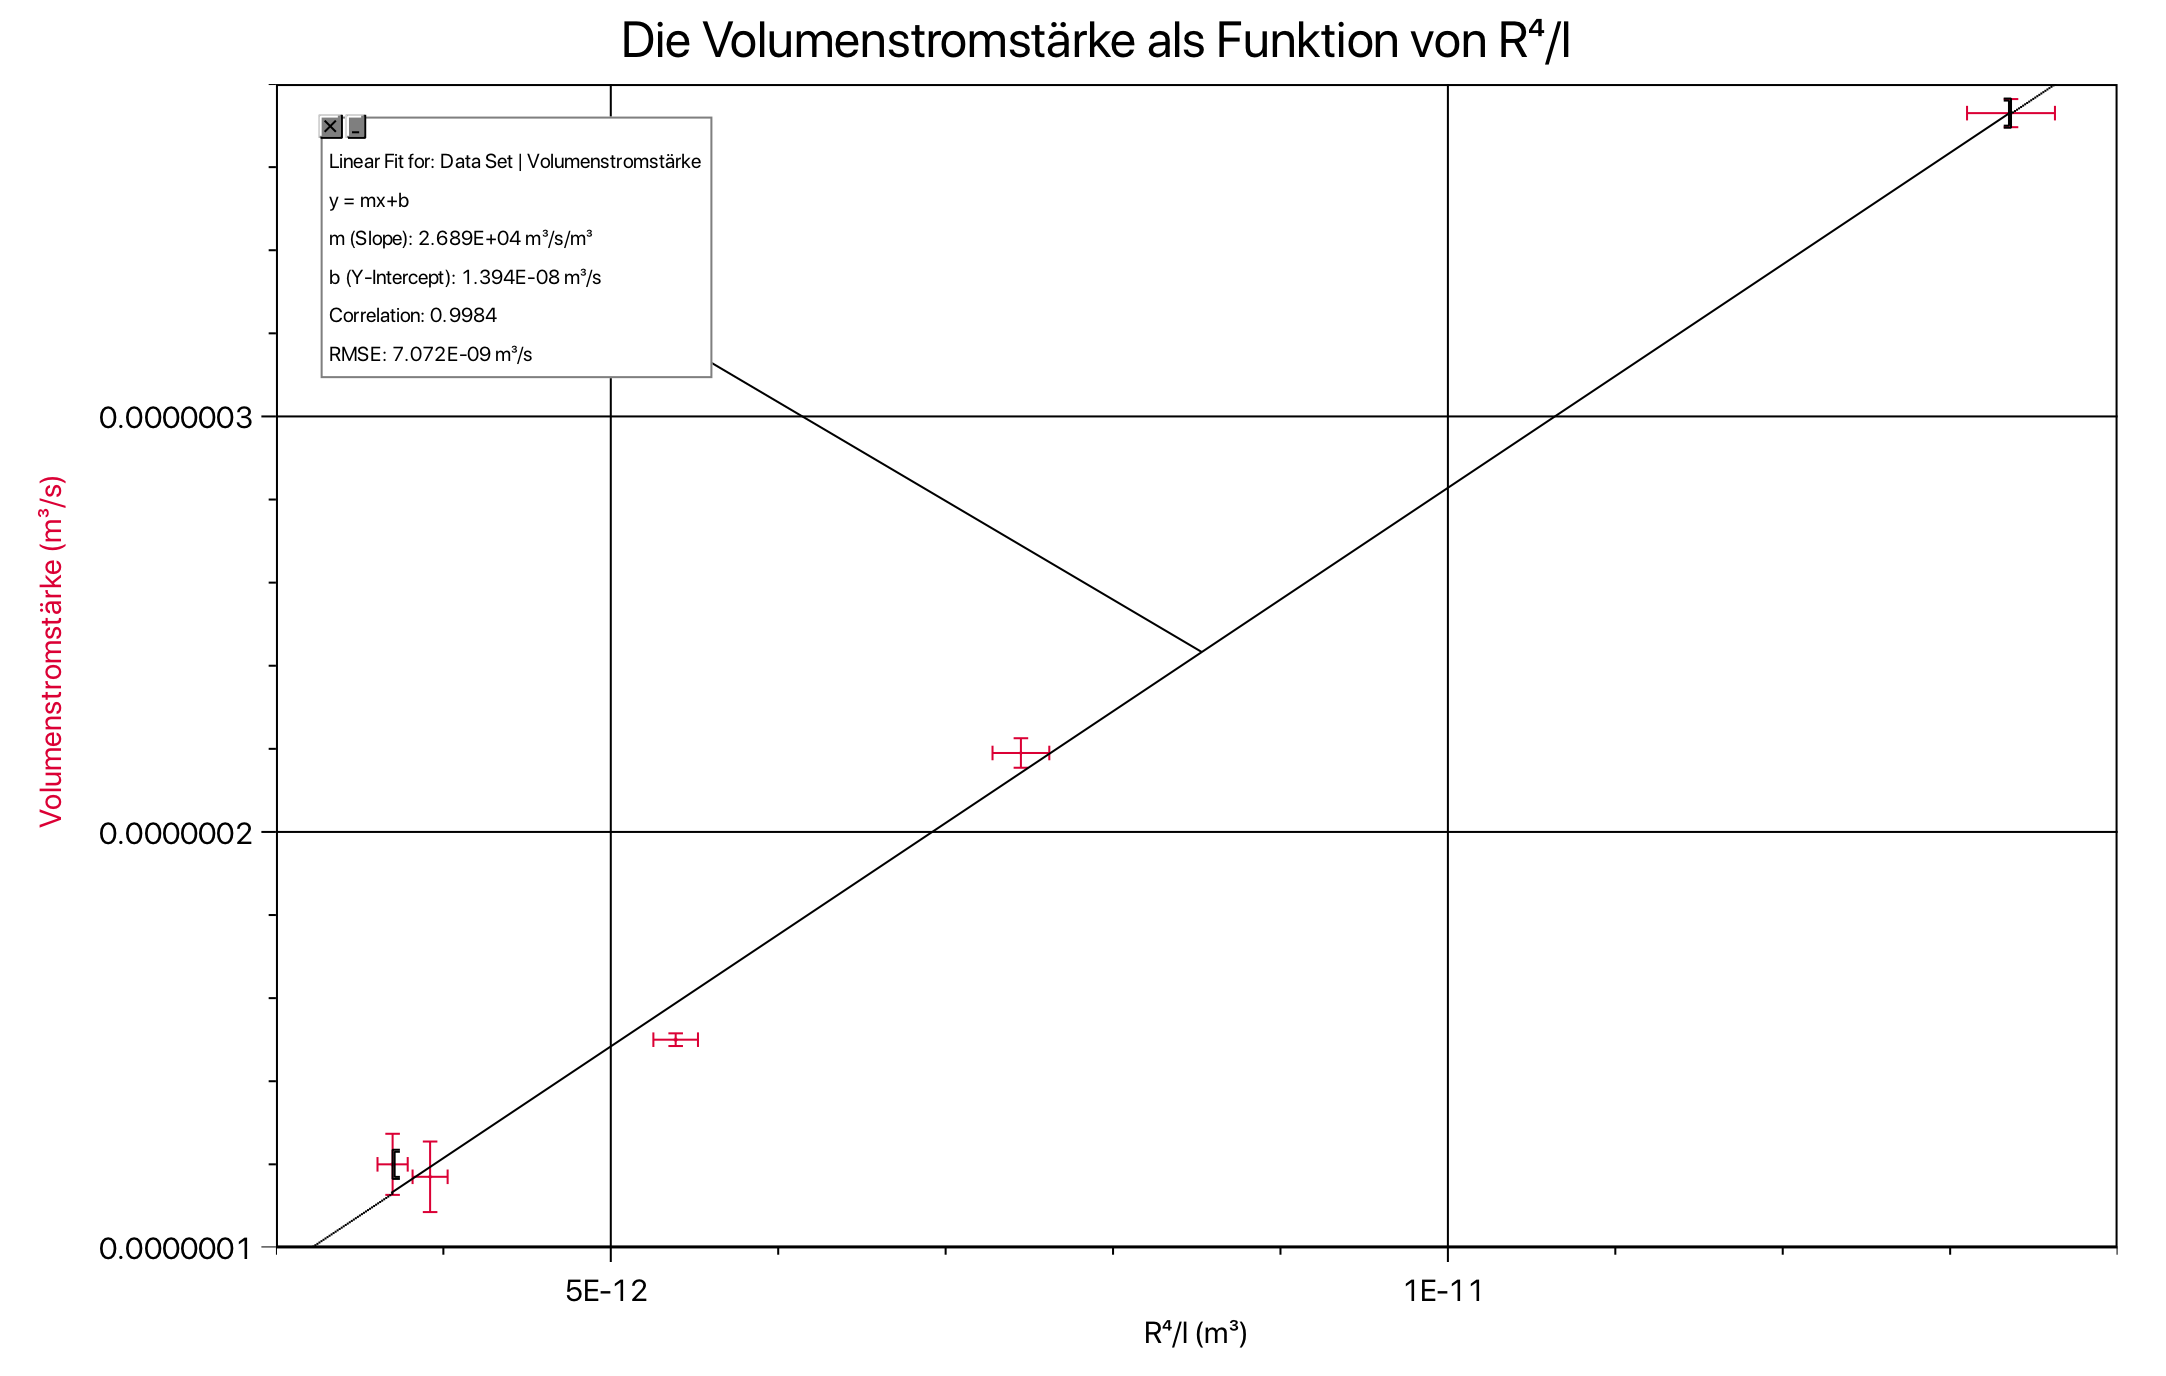
\includegraphics[width=\linewidth]{Abb2}
	\caption{Die Volumenstromstärke als Funktion von $\frac{R^4}{l}$ sowie die berechnete Ausgleichsgerade}
\end{figure}

Die lineare Regression lautet:
$$ I_V = 1,4\cdot 10^{-8} + 430000 (\frac{R^4}{l})$$

Mit den Unsicherheiten $u_a = 7\cdot 10^{-9}$ m$^3$/s und $u_b = 10000$ s$^{-1}$. 

\begin{tcolorbox}[colback=white]
	\subsection{Rechenweg}
	Die Einzelne Messwerte wurden gemittelt und in die Graph aufgetragen. Für die Unsicherheit wurde die Standardunsicherheit, oder die Standardabweichung benutzt:
	$$s_x = \sqrt{\frac{\sum_{i=1}^{n}(x_i-\bar{x})^2}{n-1}} $$
	
	Die Werte für $a$ und $b$ sowie deren Unsicherheiten lassen sich mit den folgenden Formeln bestimmen:
	$$a = \frac{
	\sum x_i^2 \sum y_i - \sum x_i \sum x_iy_i
}{
n \sum x_i^2 - (\sum x_i)^2
}$$
$$ b = \frac{
n\sum x_iy_i-\sum x_i \sum y_i
}{
n \sum x_i^2 - (\sum x_i)^2
}$$

$$u_a = s\cdot \sqrt{
\frac{
\sum x_i^2
}{
n\sum x_i^2 - (\sum x_i)^2
}}$$

$$u_b = s\cdot \sqrt{
\frac{
n
}{
n\sum x_i^2 - (\sum x_i)^2
}}$$
Mit $x = \frac{R^4}{l}$, $y = I_V$ und $s = \sqrt{
\frac{1}{n-2}\sum [y_i-(a+bx_i)]^2}$
\end{tcolorbox}

Mit der Steigung kann der Wert für $\eta$ berechnet werden. 
$$\eta = \frac{\pi \rho_w hg}{8b}$$
$$ = (0,00100 \pm 0,00002) \textrm{Pa s} $$

\begin{tcolorbox}[colback=white]
\subsection{Rechenweg}
Zur Bestimmung der Unsicherheit von $\eta$ wurde die vereinfachte gauß'sche Fehlerfortpflanzung für Produkte und Quotienten benutzt. Deswegen ist:
$$\left\vert \frac{u_\eta}{\eta} \right \vert 
= \sqrt{(\frac{u_h}{h})^2+(\frac{u_b}{b})^2} $$
(Die Unsicherheit von $h$ wurde mit der Standardunsicherheit berechnet.)
	
\end{tcolorbox}


\section{Diskussion der Ergebnisse}

\section{Literatur}

	
	
	
	
	
	
	
	
	
	
	
	
\end{document}